% !TEX encoding = UTF-8 Unicode

As instruções da MVN podem ser resumidas pela tabela da figura~\ref{fig:instrucoes-mvn}.

\begin{figure}[ht]
	\centering
	\caption{Lista de instruções da MVN}
	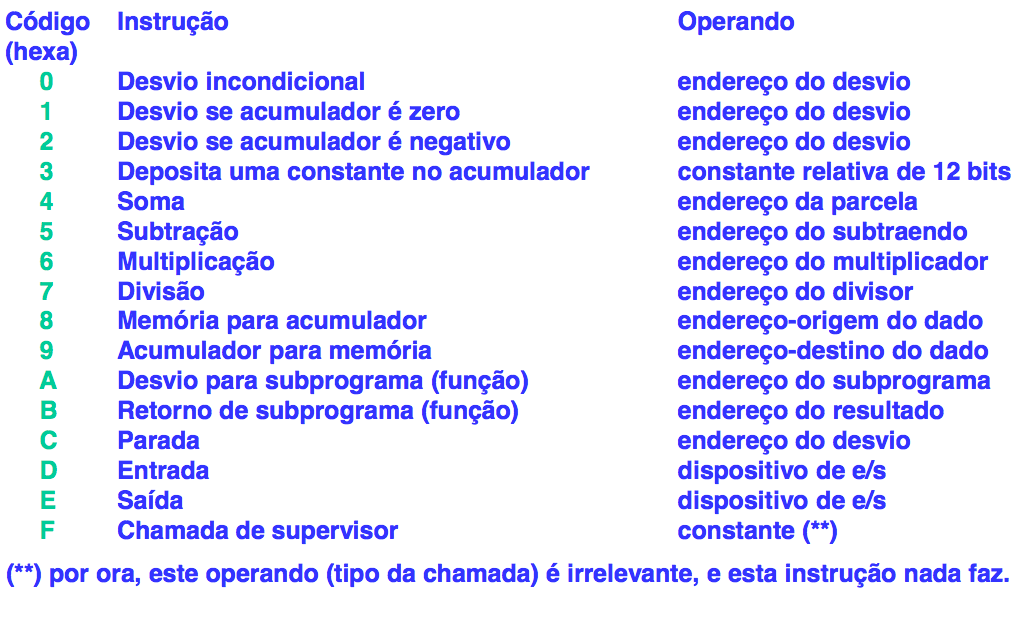
\includegraphics[width=\textwidth]{images/instrucoes-mvn.png}
	\label{fig:instrucoes-mvn}
\end{figure}

A seguir, especificaremos o que é realizado pela máquina ao executar cada tipo de operação.		

\begin{itemize}
	\item Registrador de instrução = 0 (desvio incondicional)

	Modifica o conteúdo do registrador de Endereço da Próxima Instrução (IC) armazenando nele o conteúdo do registrador de operando (OI)

	IC := OI

	\item Registrador de instrução = 1 (desvio se acumulador é zero)

	Se o conteúdo do acumulador (AC) for zero, então modifica o conteúdo do registrador de Endereço da Próxima Instrução (IC), armazenando nele o conteúdo do registrador de operando (OI) 

	Se AC = 0 então IC := OI 
	
	Se não IC := IC + 1 

	\item Registrador de instrução = 2 (desvio se negativo)

	Se o conteúdo do acumulador (AC) for negativo, isto é, se o bit mais significativo for 1, então modifica o conteúdo do registrador de Endereço da Próxima Instrução (IC) armazenando nele o conteúdo do registrador de operando (OI)

	Se AC < 0 então IC := OI 
	
	Se não IC := IC + 1

	\item Registrador de instrução = 3 (constante para acumulador)

	Armazena no acumulador (AC) o número relativo de 12 bits contido no registrador de operando (OI), estendendo seu bit mais significativo (bit de sinal) para completar os 16 bits do acumulador
		
	AC := OI 
	
	IC := IC +1 

	\item Registrador de instrução = 4 (soma)

	Soma ao conteúdo do acumulador (AC) o conteúdo da posição de memória indicada pelo registrador de operando MEM[OI]. Guarda o resultado no acumulador

	AC := AC + MEM[OI] 

	IC := IC + 1

	\item Registrador de instrução = 5 (subtração)

	Subtrai do conteúdo do acumulador (AC) o conteúdo da posição de memória indicada pelo registrador de operando MEM[OI]. Guarda o resultado no acumulador

	AC := AC - MEM[OI]

	IC := IC + 1 
		
	\item Registrador de instrução = 6 (multiplicação)

	Multiplica o conteúdo do acumulador (AC) pelo conteúdo da posição de memória indicada pelo registrador de operando MEM[OI]. Guarda o resultado no acumulador

	AC := AC * MEM[OI] 

	IC := IC + 1

	\item Registrador de instrução = 7 (divisão inteira)

	Dividir o conteúdo do acumulador (AC) pelo conteúdo da posição de memória indicada pelo registrador de operando MEM[OI]. Guarda a parte inteira do resultado no acumulador

	AC := int (AC / MEM[OI])

	IC := IC + 1 
			
	\item Registrador de instrução = 8 (memória para acumulador)

	Armazena no acumulador (AC) o conteúdo da posição de memória endereçada pelom registrador de operando (OI) 

	AC := MEM[OI]		

	IC := IC + 1
			
	\item Registrador de instrução = 9 (acumulador para memória)

	Guarda o conteúdo do acumulador (AC) na posição de memória endereçada pelo registrador de operando (OI) 

	MEM[OI] := AC		
	
	IC := IC + 1 
			
	\item Registrador de instrução = A (desvio para subprograma)

	Armazena o conteúdo do registrador de Endereço da Próxima Instrução (IC), incrementado de uma unidade, no registrador de endereço de retorno (RA). Armazena no registrador de Endereço da Próxima Instrução (IC) o conteúdo do registrador de operando (OI).

	RA := IC + 1
	
	IC := OI

	\item Registrador de instrução = B (retorno de subprograma)

	Armazena no registrador de Endereço da Próxima Instrução (IC) o conteúdo do registrador de endereço de retorno (RA), e no acumulador (AC) o conteúdo da posição de memória apontada pelo registrador de operando (OI) 

	AC := MEM[OI]			

	IC := RA 	 	 	 		

			
	\item Registrador de instrução = C (stop)

	Modifica o conteúdo do registrador de Endereço da Próxima Instrução (IC) armazenando nele o conteúdo do registrador de operando (OI) e para o processamento

	IC := OI

	\item Registrador de instrução = D (input)
 					
	Aciona o dispositivo padrão de entrada e aguardar que o usuário forneça o próximo dado a ser lido. Transfere o dado para o acumulador 

	Aguarda
	
	AC := dado de entrada 
	
	IC := IC + 1 
		
	\item Registrador de instrução = E (output)

	Transfere o conteúdo do acumulador (AC) para o dispositivo padrão de saída. Aciona o dispositivo padrão de saída e aguardar que este termine de executar a operação de saída 

	dado de saída := AC 

	aguarda
	
	IC := IC + 1

	\item Registrador de instrução = F (supervisor call)

	Não implementado: por enquanto esta instrução não faz nada.

	IC := IC + 1
\end{itemize}

Escrever um programa usando diretamente codificação binária não é uma tarefa simples, e tampouco agradável. Naturalmente, se um programa é muito grande ou se lida com diversas estruturas complexas (listas, etc.), a sua codificação se torna ainda mais difícil e complexa.

Por conta disso, torna-se imprescindível construir alguma abstração que facilite a programação e a verificação dos programas. A primeira idéia, mais natural, é utilizar o modelo de máquina existente e, a partir dele, definir nomes (mnemônicos) para cada instrução da máquina. Posteriormente, verifica-se que somente isso não basta, pois é necessário lidar com os endereços dentro de um programa (rótulos, operandos, sub-rotinas), com a reserva de espaço para tabelas, com valores constantes. Enfim, é necessário definir uma linguagem simbólica.

\begin{figure}[ht]
	\centering
	\caption{Esquema geral de um montador}
	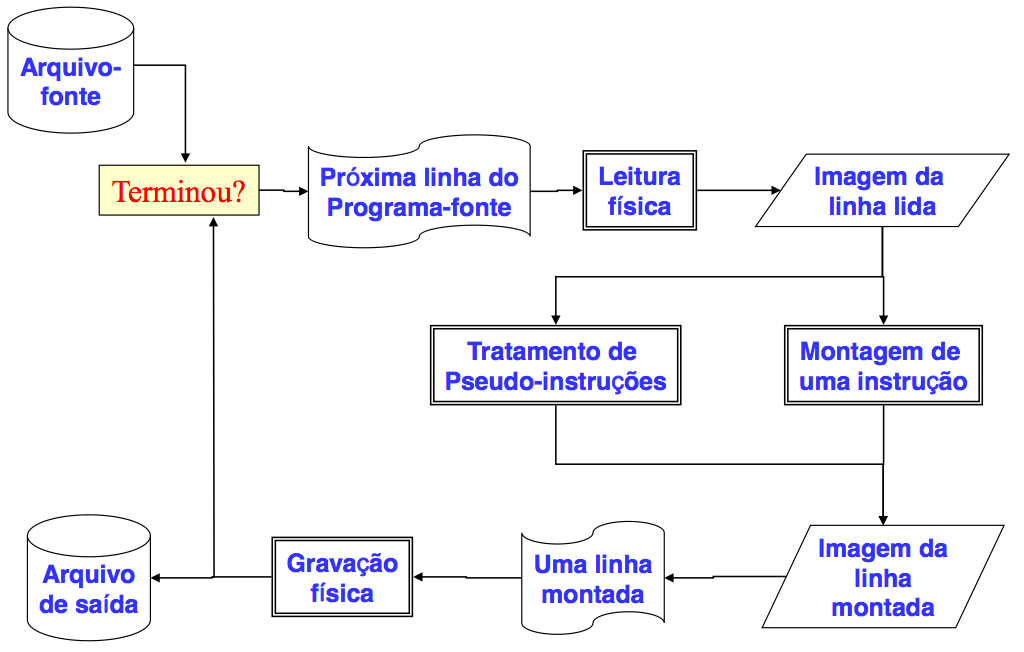
\includegraphics[width=\textwidth]{images/esquema-montador.png}
	\label{fig:esquema-montador}
\end{figure}

Para a construção de um montador, cujo esquema geral está representado na figura~\ref{fig:esquema-montador} pressupõe-se que sejam tratadas as seguintes questões:

\begin{itemize}
	\item definição das instruções: determinar os mnemônicos que as representam simbolicamente;
	\item definição das pseudo-instruções: determinar os mnemônicos que as representam, bem como sua função para o montador.
\end{itemize}

As instruções para a MVN são apresentadas na figura~\ref{fig:mnemonicos-mvn}.

\begin{figure}[ht]
	\centering
	\caption{Tabela de mnemônicos para a MVN (de 2 caracteres)}
	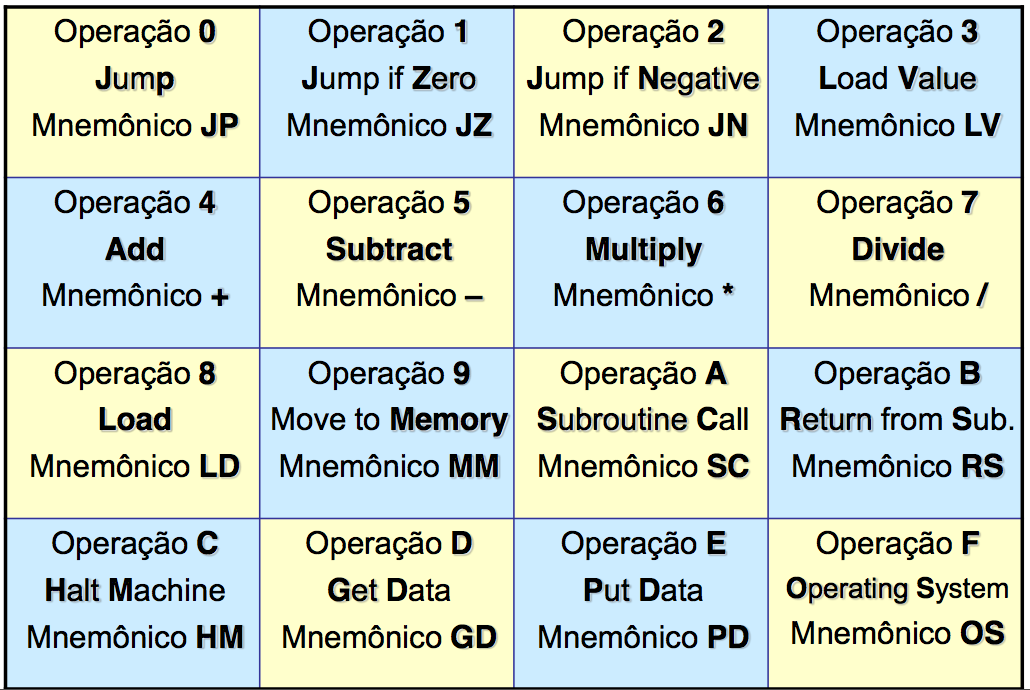
\includegraphics[width=\textwidth]{images/mnemonicos-mvn.png}
	\label{fig:mnemonicos-mvn}
\end{figure}
